\textbf{Граф хранится в специальном классе со следующими полями:}

\begin{itemize}
    \item Вершины графа хранятся списком:
    \[ V_G = (x_1, x_2, \ldots, x_k) \]
    где $k$ - количество вершин графа, $x_i$ - координата $i$-ой вершины
    
    \item Рёбра графа хранятся множеством:
    \[ E_G = \{(a_1, b_1), (a_2, b_2), \ldots\} \]
    где $a_i < b_i$ - номера вершин
    
    \item Также хранится объект \texttt{NetworkX.Graph} для удобного использования различных алгоритмов на графах
\end{itemize}

\textbf{Класс имеет 3 метода:}
\begin{enumerate}
    \item Два метода для построения рёбер, соответствующих:
    \begin{itemize}
        \item KNN-графу
        \item Distance-графу
    \end{itemize}
    \item Один метод для визуализации графа
\end{enumerate}


\textbf{Ниже приведена UML-диграмма класса}\\
\begin{center}
    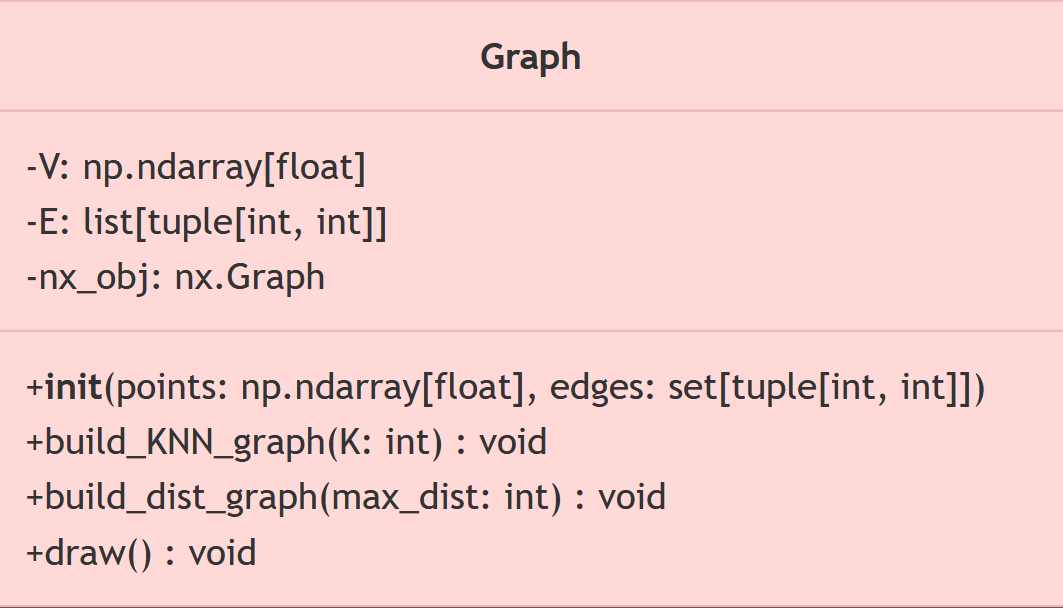
\includegraphics[width=0.6\textwidth]{graphs_implementation/UML graph.png}\\    
\end{center}

